\subsection{Arcos y homotopías}
\begin{definicion}[Arco]
  Un arco en el espacio \(X\) es una función continua \(f : I \to X \)
  donde \(I = [0,1]\)
\end{definicion}
%% mariela: q1 ¿todo espacio 1-dimensional es homeomorfo a [0,1]?
%% no dije exactamente eso, un subconjunto convexo y acotado si lo es ,
%% pero debo de preguntar que se refiere
La definición tradicional es ligeramente mas general, cambiando que \(I\)
sea un subconjunto convexo acotado de un espacio unidimensional, pero
siempre podemos recuperar esta definición re-escalando la distancia.

\begin{definicion}[Homotopía]
  Dados dos arcos \(f,g : I \to X\), diremos que \(f\) es homotópico a
  \(g\) si existe una función continua \(F : I \times I \to X \) tal que
  \[ \begin{matrix}
      F (x, 0) = f(x), & F (x, 1) = g(x)
     \end{matrix}
  \]
  Donde \(F\) sera llamada una homotopía entre \(f\) y \(g\). La
  existencia de dicha relación entre dos funciones sera denotada por \(f
  \homRelAlt g\).
\end{definicion}
\begin{figure}[h]
  \centering
  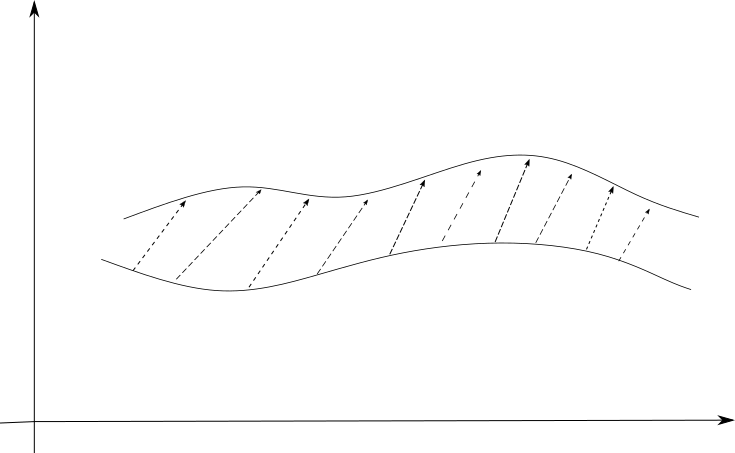
\includegraphics[scale=0.3]{./imagenes/homotopia.png}
  \caption{caracterización homotopía}
  \label{fig:homotopia-entre-funciones}
\end{figure}
Podemos pensar en el segundo argumento de una homotopía como el grado de
deformación entre dos funciones.
Si tratamos con arcos \(f,g : I \to X\) que posean los mismos puntos
iniciales y finales, es decir \(f(0) = g(0) = x_0, \; f(1) = g(1) =
x_1 \) podemos definir una relación homotópica ligeramente mas fuerte.

\begin{definicion}[Arco homotopía] \label{def:arco-homotopia}
  \(f,g : I \to X\) son \emph{arco homotópicas} entre sí, si tienen los mismos
  puntos inicial y final \(x_0, x_1\) respectivamente y existe una homotopía entre
  ellos tal que cumpla
  \[
    \begin{matrix}
      F(s,0) = f(s), & F(s,1) = g(s) & ~ \\
      F(0,t) = x_0,  & F(1,t) = x_1, & \forall t \in I
    \end{matrix}
  \]
  La existencia de esta relación entre dos funciones sera denotada por
  \(f \simeq g\).
\end{definicion}
% todo(slack) hacer algun dibujo de las homotopías entre las curvas
Una vez definida estas relaciones, una pregunta natural es si estas definen
una relación de equivalencia, ya que nos gustaría identificar clases de
curvas como elementos de alguna teoría algebraica. La respuesta es
afirmativa para ambas relaciones (el punto de inicio y final no juegan
un papel relevante). A continuación mostraremos que ``ser homotópicas''
es una relación de equivalencia.
\begin{teorema}
  \(\homRelAlt\) es una relación de equivalencia
\end{teorema}
\begin{proof}
  Hemos de probar que esta relación cumple la reflexividad, simetría y
  transitividad. Sean \(f,g,h : I \to X\) tres arcos arbitrarios.
  \begin{itemize}
  \item La reflexividad es directa pues la función \(F(x,t) = f(x)\) es
    una deformación continua de \(f\) a \(f\), por tanto \(f \homRelAlt
    f\).

  \item La simetría se obtiene de invertir el sentido de deformación de la
    homotopía original. Formalmente, dado \(f \stackrel{.}{\simeq} g\)
    tenemos una homotopía \((x,t) \mapsto F(x,t)\) entre estas. A partir
    de aquí podemos definir
    \begin{equation}
      \label{eq:homotopy-simetry}
      (x,t) \mapsto \hat{F}(x,t) := F(x,1-t)
    \end{equation}
    con \(\hat{F}\) una homotopía entre \(g\) y \(f\). Por tanto \(g
    \stackrel{.}{\simeq} f\).

  \item La transitividad se obtiene a partir de parametrizar \(I\) en dos
    intervalos donde se deformen individualmente cada homotopía al doble
    del grado. Formalmente dado \(f \stackrel{.}{\simeq} g\) y \(g
    \stackrel{.}{\simeq} h\) representadas por las homotopías \(F\) y
    \(G\) respectivamente, se define
    \[ FG(x,t) = \begin{cases}
        F(x,2t) & t \in [0,\frac{1}{2}] \\
        G(x,2t - 1) & t \in [ \frac{1}{2} , 1]
      \end{cases}
    \]
    Esta es una deformación continua claramente en \((x,t) \in I \times
    [0, \frac{1}{2}) \cup I \times (\frac{1}{2}, 1]\). La continuidad en
    \(I \times \{\frac{1}{2}\}\) proviene de la consistencia en dicho
    punto de ambas homotopías
    \[ F(x,2 \cdot \frac{1}{2}) = g(x) = G(x, 2 \cdot \frac{1}{2} - 1)\]
    lo que nos permite utilizar el \emph{lema del pegamiento}
    \cite[p.~108]{munkres} para obtener la continuidad de \(FG\).
    Obteniendo así \(f \stackrel{.}{\simeq} h\).
  \end{itemize}
\end{proof}

En análisis real, es común trabajar con conjuntos convexos. En arcos
sobre estos conjuntos, veremos una homotopía repetidamente llamada
homotopía de linea recta.
\begin{definicion}[Homotopía de linea recta]\label{def:homotopia-linea}
  Sean \(f,g : I \to X\) dos arcos arbitrarios y sea \(\mathcal C
  \subset X\) un subconjunto convexo. Si \(f(I),g(I) \subset \mathcal
  C\), entonces se define la homotopía de linea recta por
  \[ F(x,t) := (1-t) \cdot f(x) + t \cdot g(x) \]
\end{definicion}
\begin{acotacion}
  En la definición anterior, la continuidad de \(F\) se obtiene de ser
  una combinación convexa de funciones continuas \(f\) y \(g\). Por ser
  una combinación convexa, se requiere pedir la existencia de un conjunto
  \(\mathcal C \subset X\) que contenga a las imágenes de dichas
  funciones. Pues de no ser así, podríamos obtener que la imagen no este
  definida en el espacio topológico.
\end{acotacion}

Con estas definiciones ya podemos empezar a hablar de clases
de equivalencia de funciones bajo una relación homotópica
\[ [f] = \{ g : I \to X \mid f \stackrel{.}{\simeq} g \} \]
Notar que la construcción anterior es valida para las dos relaciones,
aunque por nuestra meta de construir el grupo fundamental nos interesa
principalmente la relación arco homotópica, por razones a estudiar mas
adelante.
